
Our program is written in the programming language Python. We made that decision because that is the program we are all familiar with and will all be able to understand the code. 

\subsection{Data storage}

Tasks are implemented as objects, where each one has it is own 
\begin{itemize}
    \item \texttt{name}, stating the name of the task,
    \item \texttt{duration}, meaning the time it takes for the task,
    \item \texttt{required task-prerequisites}, which is a list of tasks-names that have to be completed before,
    \item \texttt{required resources}, meaning all items needed for the task
    for instance \textit{cooking stove, knife, cook}
\end{itemize}
Our recipes are portrayed as lists of tasks and saved in a separate \texttt{json file}. The kitchen resources are also defined in another \texttt{json file}, where each one is assigned a \texttt{name} and \texttt{num}, meaning quantity. \\
A few parameters are set at the start of the code. These are the recipe file and the difference of time factor, which we will talk more about later.
To save the data, that is changing throughout the cooking process, we constricted a class cooking, where we define these properties:
\begin{itemize}
    \item list of completed tasks, which is at first empty, later on we will add the completed tasks here,
    \item list of resources, imported from the json file,
    \item list of tasks, also imported from the json file,
    \item copy of list of tasks, that will not change throughout the simulation,
    \item order, where we save the order of tasks in current simulation.
\end{itemize}

\subsection{Recipe Simulation}

For the actual simulation, meaning for a recipe to be excecuted, we defined another class named DiscreteEventSimulator. 
Everytime we construct a new one, we also construct a new class cooking. This way all our parameters are everytime set back to the start (ex. list of completed tasks).
The class also has a parameter \texttt{event\_queue}, where scheduled events are being added, and parameter \texttt{time}. \\

\begin{figure}[H]
    \centerline{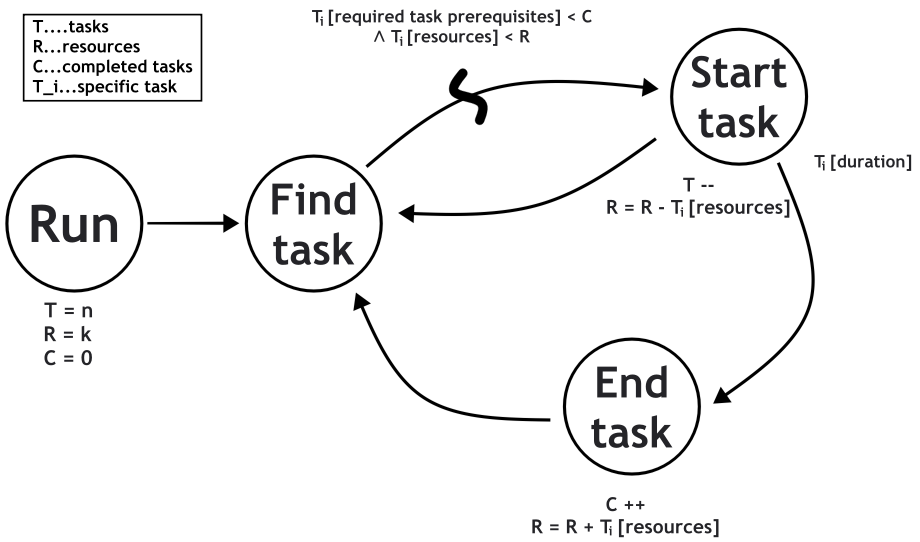
\includegraphics[scale=.4]{/Users/lanar/Documents/Cooking-model/Documentation/images/graph.png}}
    \caption{Discrete simulation graph of a cooking process.}
    \label{fig1}
\end{figure}

On this figure \ref{fig1}, we can see a simplified graph on how the simulation works. We start by calling the method \texttt{find\_task}, this as suggested searches for a task that can be executed, meaning all resources needed are available 
and all tasks, that needed to be done before, are already completed. If we find such a task, method \texttt{start\_task} is called, where the previously mentioned resources are taken of the list, the task name is added to the order and the method \texttt{schedule\_end\_task} is invoked. 
There we make an event, where we calculate the time when it will be finished by adding up duration to 'current time' and save the name of the task. This is appended to the \texttt{event\_queue} list. Directly after, the method \texttt{find\_task} is executed again. \\ 

Right at the start we start a while loop, that will be done once. The number of completed tasks is the same as the number of tasks at the start. 
With each iteration of the loop, the time increases by one. We also use this to check if there is an event scheduled at the current time. In case there is one we call the method \texttt{end\_task}. 
This is where the previously removed resources are added back to the list and the task is added to the list of completed tasks. 

At the end the function \texttt{run\_simulation} returns a tuple, where the first component is the time it took, and the second the order in which the tasks were completed. 
In case the you one does not have the required resources needed for the recipe, the program returns the error: \texttt{You do not have the right resources}.

Now that we got our program to execute a recipe, we started to work on finding the optimal ordering of tasks, to get the shortest time. 

\subsection{Different orders of tasks}
The first idea we got, was just to try all possible permutations of the list of tasks. Run the simulation for each one of them and then choose the one with the shortest time.
To help with understanding the code and making sure it worked well, we made sure to get a list of all possible orders and the time it took. Furthermore due to prior task prerequisites the recipe we had at the start returned us the same duration, no mater the order of tasks. 
To fix it we added a task, to have a three-task process, meaning heating the water, peeling potatoes and cooking them. Moreover, we changed some of the durations of tasks. 

When running the code we realized, that the order of the last few tasks rarely changes. This was caused by the prior task prerequisites, since these tasks can only be done once the others are completed.
Below you can see some of the possible orders we got. 

\begin{verbnobox}[\fontsize{8pt}{8pt}\selectfont]
[cutting meat, heating water, cutting onions, cooking meat, frying onions, cooking potatoes, cooking everything] 
[cutting meat, cutting onions, heating water, cooking meat, frying onions, cooking potatoes, cooking everything] 
[heating water, cutting meat, cutting onions, cooking meat, frying onions, cooking potatoes, cooking everything] 
[heating water, cutting onions, cutting meat, cooking meat, frying onions, cooking potatoes, cooking everything] 
[cutting onions, cutting meat, heating water, cooking meat, frying onions, cooking potatoes, cooking everything] 
[cutting onions, heating water, cutting meat, cooking meat, frying onions, cooking potatoes, cooking everything] 
\end{verbnobox}

This gave us the idea, that instead of testing all possible orders, we should firstly check which tasks are required to be done first and put those at the start of the list. 
Furthermore, the ones, who are required for more tasks, should be done first, meaning put at the start of the list, and others, which are not required for any task, should be left behind.
With this in mind we wrote the function \texttt{smart\_permutations}, which takes the name of the recipe json file and returns some permutations of the tasks, where we know one of them will give us the best order. 
Here we can see the simplified process:

\begin{verbnobox}
- get tasks from json file
- for task in all tasks:
    get task prerequisites (can be repeated)
- count repetitions of tasks
- sort in lists based on number of repetitions
- get all other tasks
- permutate each task list separately
- make all possible combinations 
\end{verbnobox}

This is afterwards inputed into the function \texttt{run}, which tries all the given orders and returns the one with the shortest duration. 


\subsection{Introducing randomness}
Since cooking does not always go as planned, we added some randomness, by prolonging/shortening the duration of tasks. 
We started by defining a parameter \texttt{time\_change\_factor} at the start of the code, which states for maximum, how many 'seconds' can a task be prolonged or shortened. 
This is all done in the function \texttt{time\_randomness} that is called when scheduling a task and calculating the time it will be completed. 
The following graph of our simulation is on figure \ref{fig2}, where the function \textit{f} represents the previously mentioned function. 

\begin{figure}[H]
    \centerline{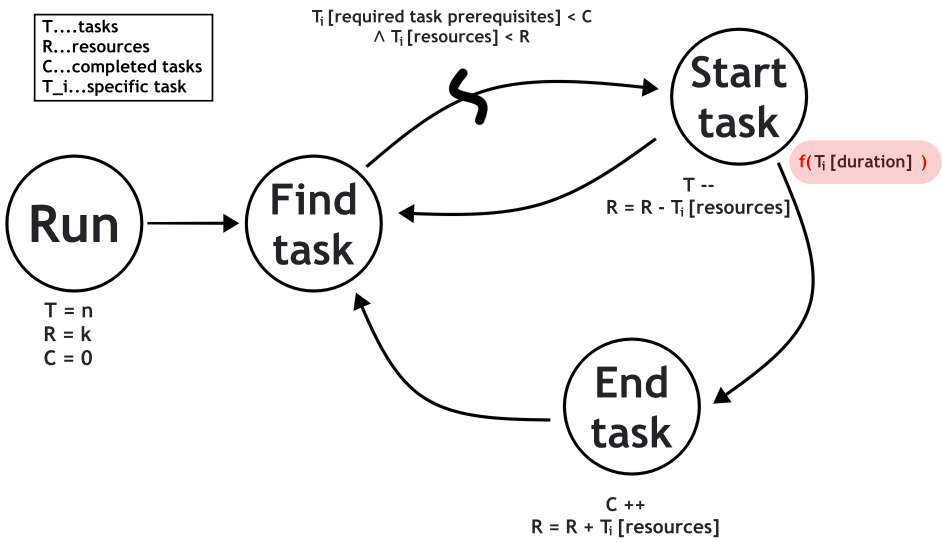
\includegraphics[scale=.23]{/Users/lanar/Documents/Cooking-model/Documentation/images/graph_showing_time.png}}
    \caption{Discrete simulation graph of a cooking process with time randomness.}
    \label{fig2}
\end{figure}


